
%(BEGIN_QUESTION)
% Copyright 2009, Tony R. Kuphaldt, released under the Creative Commons Attribution License (v 1.0)
% This means you may do almost anything with this work of mine, so long as you give me proper credit

Identify all values of $x$ where the derivative of the function has a value of $-1$:

$$\includegraphics[width=15.5cm]{i04297x01.eps}$$

\vfil 

\underbar{file i04297}
\eject
%(END_QUESTION)





%(BEGIN_ANSWER)

This is a graded question -- no answers or hints given!

%(END_ANSWER)





%(BEGIN_NOTES)

The general principle to keep in mind here is that derivative is the slope of the tangent line at a specified point.  Therefore, in this problem we are looking for points on the function where the tangent line will have a -1 slope:

$$\includegraphics[width=15.5cm]{i04297x02.eps}$$

$${df(x) \over dx} = -1 \hbox{ when } x \approx 7.25$$

$${df(x) \over dx} = -1 \hbox{ when } x \approx 9.85$$

Some might argue that the two corners at $x=16$ are alternative locations where the derivative passes through a value of -1.  According to mathematical convention, ``step'' functions such as the horizontal-to-vertical transition at $x=16$ are non-differentiable.  However, if this were a real-life application where $x$ was actually {\it time}, the signal would very briefly experience a slope of -1 as it transitioned from a slope of 0 to a strong negative slope, and again as it transitioned from a near-vertical slope to a negative slope less than -1.

%INDEX% Mathematics, calculus: integration (numerical)

%(END_NOTES)


